\section{Variabili Aleatorie Continue}

Rimuoviamo ora l'ipotesi che lo spazio dei campioni $\Omega$ sia discreto. D'ora in poi, supporremo che $\Omega \subseteq \mathbb{R}$ sia un sottoinsieme \textit{continuo} dei numeri reali.

In questo contesto, $\Omega$ può rappresentare direttamente lo spazio delle grandezze fisiche misurabili, oppure può fungere da dominio per un'applicazione:

\begin{equation}
X : \omega \in \Omega \longrightarrow X(\omega) \in \mathcal{X}
\end{equation}

Naturalmente, l'alfabeto $\mathcal{X}$ non è più vincolato a essere un insieme finito o numerabile; molto spesso, inoltre, accade che $X(\omega) = \omega$ e, di conseguenza, $\mathcal{X} = \Omega$.

Per chiarire la differenza con il caso discreto, ripensiamo all'esperimento del lancio di una moneta:
\begin{itemize}
    \item \textit{Esperimento}: Lancio di una moneta.
    \item \textit{Esito $\omega$}: "Testa" o "Croce". Essendo stringhe testuali e non numeri, lo spazio campionario è $\Omega = \{\text{Testa}, \text{Croce}\}$.
    \item \textit{Intervento di $X$}: La variabile aleatoria funge da "ponte", mappando gli esiti in valori numerici: $X(\text{Testa}) = 1$ e $X(\text{Croce}) = 0$.
    \item \textit{Alfabeto $\mathcal{X}$}: È l'insieme dei possibili valori assunti, ovvero $\{0,1\}$.
\end{itemize}

Nel caso discreto, l'esito base $\omega$ ("Testa") era profondamente diverso dal suo valore mappato $X(\omega)$ ("1"). Nel caso continuo, invece, \textbf{$\Omega$ è già costituito da numeri}, trattandosi di un sottoinsieme dei reali.

Il passaggio dal discreto al continuo richiede un adattamento nel calcolo delle probabilità. La definizione frequentista utilizzata finora smette di funzionare:

\begin{equation}
\mathbb{P}(X = x_i) = \lim_{n \to \infty} \frac{n_{X=x_i}}{n}
\end{equation}

L'idea di "ripetere l'esperimento infinite volte e contare quante volte appare esattamente $x_i$" non è più applicabile: essendo l'alfabeto continuo e infinito, la probabilità di centrare un singolo valore esatto perde di significato.

\subsection{Probabilità su un Intervallo}

Immaginiamo di dover misurare una grandezza continua, come la tensione elettrica o la temperatura. 
Supponiamo che la prima misurazione restituisca il valore \textbf{$22.45719385\dots^\circ C$} (con infiniti decimali). 

Qual è la probabilità che, effettuando una seconda misurazione, la temperatura risulti \textit{esattamente identica} alla prima? Nel mondo reale, per registrare due valori assolutamente identici, servirebbe uno strumento a precisione infinita, che non esiste. 

Per aggirare questo ostacolo matematico e concettuale, introduciamo l'uso degli \textbf{intorni}.
Invece di chiederci: \textit{``Qual è la probabilità di misurare esattamente $22.00000^\circ C$?''}, 
cambiamo prospettiva e ci domandiamo: \textit{``Qual è la probabilità che la temperatura ricada nell'intervallo tra $21.9^\circ C$ e $22.1^\circ C$?''}

Da qui ricaviamo la prima regola:
\begin{quote}
\textbf{Per una variabile aleatoria continua, la probabilità di osservare un singolo valore esatto è SEMPRE NULLA.} Matematicamente si scrive: $\mathbb{P}(X=x) = 0$.
\end{quote}

Calcoliamo quindi la probabilità su un intorno. Ipotizziamo di compiere $n$ esperimenti, raccogliendo un set di osservazioni $\{X(\omega_i)\}$ per la variabile continua $X$. 
Dato un valore di interesse $x \in \mathcal{X}$, vogliamo calcolare la frequenza con cui i risultati cadono in un intorno di ampiezza $\Delta x$ centrato in $x$:

\begin{equation}
f_n(x; \Delta x) = \frac{n_{\left\{x - \frac{\Delta x}{2} \le X \le x + \frac{\Delta x}{2}\right\}}}{n}
\end{equation}

Analizziamo i termini dell'intervallo:
\begin{itemize}
    \item \textbf{$x$}: È il "centro bersaglio", il valore nominale che ci interessa (es. $22^\circ C$).
    \item \textbf{$\Delta x$}: È l'ampiezza totale della "finestra di tolleranza" (es. $0.2^\circ C$).
    \item Suddividendo la tolleranza a metà ($\pm \frac{\Delta x}{2}$), costruiamo un intervallo perfettamente centrato su $x$.
\end{itemize}

Il numeratore della formula rappresenta semplicemente il conteggio delle osservazioni che, su $n$ prove, soddisfano la condizione $x - \frac{\Delta x}{2} \le X(\omega) \le x + \frac{\Delta x}{2}$.

Se immaginassimo di ripetere l'esperimento infinite volte ($n \to \infty$), per la legge dei grandi numeri questa frequenza convergerebbe a un valore stabile. Quel limite rappresenta la \textbf{probabilità reale} che l'evento si verifichi in quell'intervallo:

\begin{align}
\mathbb{P}\left(\omega \in \Omega : \left\{x - \frac{\Delta x}{2} \le X \le x + \frac{\Delta x}{2}\right\}\right) &= \mathbb{P}\left(X \in \left[x - \frac{\Delta x}{2}, x + \frac{\Delta x}{2}\right]\right) \nonumber \\
P_X(x; \Delta x) &= \lim_{n \to \infty} f_n(x; \Delta x)
\end{align}

\subsection{Densità di Probabilità (PDF)}

Si definisce \textbf{funzione di densità di probabilità} (Probability Density Function, PDF) di una variabile aleatoria continua $X$ il seguente limite:

\begin{equation}
\boxed{f_X(x) = \lim_{\Delta x \to 0} \frac{\mathbb{P}\left(x - \frac{\Delta x}{2} \le X \le x + \frac{\Delta x}{2}\right)}{\Delta x}}
\end{equation}

Per afferrare il senso della divisione per $\Delta x$, è utile un parallelismo con la fisica. Come si calcola la densità lineare di una sbarra di ferro? Si prende la massa di un piccolo frammento e la si divide per la sua lunghezza. 
La logica qui è identica: prendiamo la "massa di probabilità" contenuta nel nostro intervallo (il numeratore) e la dividiamo per la larghezza dell'intervallo stesso ($\Delta x$).
Facendo tendere l'ampiezza della finestra a zero tramite il limite, otteniamo la "densità" di probabilità istantanea nel singolo punto $x$.

\textbf{ATTENZIONE: La densità $f_X(x)$ NON è una probabilità}. A differenza delle probabilità, la PDF può assumere valori strettamente maggiori di 1. È semplicemente un indicatore che ci mostra quanto i risultati tendano ad "addensarsi" attorno a un determinato punto.

Per passare dal concetto di densità al calcolo effettivo della probabilità, ricorriamo al \textit{Teorema fondamentale del calcolo integrale}:

\begin{equation}
\mathbb{P}\left(x - \frac{\Delta x}{2} \le X \le x + \frac{\Delta x}{2}\right) = \int_{x - \frac{\Delta x}{2}}^{x + \frac{\Delta x}{2}} f_X(t)dt
\end{equation}

Questa formula esprime un concetto cardine: \textbf{la probabilità corrisponde all'Area}. 
Rappresentando graficamente la funzione di densità $f_X(x)$, la probabilità che un valore ricada in un dato intervallo è pari all'area sottesa alla curva in quell'intervallo. Come noto dall'analisi matematica, lo strumento per calcolare l'area sottesa a una curva è proprio l'integrale.

\subsubsection{Proprietà Fondamentali (Vincoli Costitutivi) della PDF}
Affinché una funzione possa essere considerata una valida densità di probabilità, deve soddisfare due requisiti essenziali:

\begin{itemize}
    \item \textbf{Non-negatività:} $f_X(x) \ge 0 \quad \forall x \in \mathbb{R}$. \\
    La densità non può mai assumere valori negativi. Se così fosse, calcolando l'integrale si otterrebbero "aree negative", il che porterebbe all'assurdo logico di avere probabilità minori di zero. (In termini formali, basterebbe la non-negatività \textit{quasi ovunque}).

    \item \textbf{Condizione di normalizzazione (Integrale unitario):} \\
    La funzione deve essere sommabile su $\mathbb{R}$ e l'area totale sottesa alla curva deve valere $1$:
    \begin{equation}
    \int_{-\infty}^{+\infty} f_X(t)dt = 1
    \end{equation}
    Il motivo è intuitivo: calcolare l'integrale da $-\infty$ a $+\infty$ significa prendere in considerazione \textit{tutti} i possibili esiti dell'esperimento. Poiché è certo al 100\% che la variabile assuma un valore nell'insieme dei reali, l'area totale (ovvero la probabilità dell'evento certo $\Omega$) deve essere rigorosamente pari a $1$.
\end{itemize}

\subsection{Funzione di Ripartizione (CDF)}

La \textbf{CDF} (Cumulative Distribution Function), nota in italiano come \textbf{funzione di ripartizione}, è uno strumento alternativo per caratterizzare una variabile aleatoria. 

Mentre la PDF $f_X(x)$ ci fornisce la "densità" in un punto esatto, la CDF $F_X(x)$ \textbf{accumula tutta la probabilità da sinistra verso destra}.
In termini pratici, valutare la CDF in un punto $x$ risponde alla domanda: \textit{"Qual è la probabilità che il risultato dell'esperimento sia minore o uguale a $x$?"}

\begin{equation}
F_X(x) = \mathbb{P}(-\infty < X \le x) = \int_{-\infty}^{x} f_X(t) dt
\end{equation}

Geometricamente, $F_X(x)$ rappresenta l'area totale sottesa dalla curva della PDF da $-\infty$ fino al punto $x$.

Dal momento che la CDF si ottiene integrando la PDF, per il teorema fondamentale del calcolo integrale vale anche l'operazione inversa. Se si conosce la formula della CDF e si desidera ricavare la PDF, è sufficiente calcolarne la \textbf{derivata} rispetto a $x$:

\begin{equation}
f_X(x) = \frac{d F_X(x)}{dx}
\end{equation}

\subsubsection{Probabilità in un Intervallo e CCDF}

Se desideriamo calcolare la probabilità che un valore cada all'interno di un intervallo $[a_1, a_2]$, possiamo usare direttamente la funzione di ripartizione senza dover ricalcolare l'integrale della PDF ogni volta:

\begin{equation}
\mathbb{P}(a_1 \le X \le a_2) = \int_{a_1}^{a_2} f_X(t) dt = F_X(a_2) - F_X(a_1)
\end{equation}

Esiste anche una caratterizzazione speculare detta \textbf{CCDF} (Complementary Cumulative Distribution Function). Essa risponde alla domanda opposta: \textit{"Qual è la probabilità che il risultato sia strettamente MAGGIORE di $x$?"}

Sapendo che l'area totale sotto la PDF deve valere sempre $1$ (il 100\% della probabilità), la probabilità di essere "maggiore di $x$" è semplicemente il complemento a 1 della probabilità di essere "minore o uguale a $x$":

\begin{equation}
\bar{F}_X(x) = \mathbb{P}(X > x) = \int_{x}^{+\infty} f_X(t) dt = 1 - F_X(x)
\end{equation}

\subsubsection{Proprietà della CDF}
Dalla sua definizione analitica derivano le seguenti proprietà fondamentali:
\begin{itemize}
    \item $F_X(x) \in [0, 1]$, in quanto rappresenta una misura di probabilità.
    \item $F_X(-\infty) = 0$ e $F_X(+\infty) = 1$, limiti dettati dal fatto che stiamo integrando una PDF su tutto il suo dominio.
    \item $F_X(x)$ è una funzione \textbf{continua} (essendo la funzione integrale di una funzione sommabile).
    \item $F_X(x)$ crescente: Dalla definizione sappiamo che la CDF si ottiene integrando la PDF:
    \[ F_X(x) = \int_{-\infty}^{x} f_X(t) dt \]
    Di conseguenza, sappiamo che la derivata della CDF è proprio la PDF:
    \[ \frac{d F_X(x)}{dx} = f_X(x) \]
    Sappiamo che la PDF $f_X(x)$ è una funzione sempre maggiore o uguale a 0 (perché le probabilità sono sempre comprese tra 0 e 1). Dall'analisi matematica sappiamo che se la derivata di una funzione è positiva (o nulla), allora la funzione stessa è crescente. 
    Ovvero: $\forall x_1, x_2 \in \mathbb{R}$, se $x_1 > x_2 \implies F_X(x_1) \ge F_X(x_2)$.
    Ne concludiamo che $F_X(x)$ è una funzione \textbf{monotòna non decrescente}.
    
    \item \textbf{Continuità a destra:} La CDF è continua a destra. Ovvero, se mi avvicino ad un punto $x_0$ provenendo da destra ($x_0^+$), il valore del limite che incontro è esattamente il valore della funzione in quel punto:
    \[ \lim_{x \to x_0^+} F_X(x) = F_X(x_0) \]
    In pratica, se c'è un salto nel grafico della funzione, il punto pieno (che indica il valore compreso) si trova sul segmento di destra, mentre a sinistra c'è un pallino vuoto ($\circ \!\!-\!\! \bullet$).
\end{itemize}

\subsection{Media Statistica per Variabili Continue}

Data una variabile aleatoria continua caratterizzata dalla sua PDF $f_X(x)$, definiamo il suo \textbf{valore atteso} (o media statistica) come:

\begin{equation}
\mathbb{E}[X] = \mu_X = \int_{-\infty}^{+\infty} x f_X(x) dx
\end{equation}

Questa operazione è l'esatto equivalente continuo della media per le variabili discrete ($\sum x_i p_X(x_i)$), dove la sommatoria viene sostituita dall'integrale e la probabilità puntuale viene sostituita dalla densità infinitesima $f_X(x)dx$.

\subsubsection*{Dimostrazione: Applicazione della formula al caso continuo}

Dobbiamo dimostrare che la formula classica della media statistica si applica coerentemente anche al caso continuo.

Consideriamo una variabile aleatoria continua $X$. Il primo step è \textbf{quantizzare} questa variabile. Suddividiamo l'asse delle ascisse in tanti piccoli intervalli di ampiezza $\Delta$.
In pratica, creiamo una nuova variabile quantizzata $X^\Delta$: ogni numero reale "collassa" e ti restituisce il rappresentante $x_i$ dell'intervallo in cui è caduto:
\[
X^\Delta = x_i \quad \text{per} \quad x \in [i\Delta, (i+1)\Delta[
\]

Ci chiediamo: qual è la probabilità che accada esattamente $x_i$? Dato che stiamo considerando un intervallo continuo, la probabilità per la variabile quantizzata è data dall'integrale della PDF su quell'intervallo:
\[
\mathbb{P}(X^\Delta = x_i) = \mathbb{P}(i\Delta \le X < (i+1)\Delta) = \int_{i\Delta}^{(i+1)\Delta} f_X(x) dx = p_{X^\Delta}(x_i)
\]

Ora applichiamo la definizione classica di valore atteso per la nostra variabile discreta $X^\Delta$:
\[
\mathbb{E}[X^\Delta] = \sum_{i=-\infty}^{\infty} x_i \cdot p_{X^\Delta}(x_i) = \sum_{i=-\infty}^{\infty} x_i \cdot \int_{i\Delta}^{(i+1)\Delta} f_X(x) dx
\]

Cosa succede se gli intervalli diventano infinitesimi, ovvero se $\mathbf{\Delta \to 0}$? 
Otteniamo di nuovo la nostra $X$ continua originaria. Inoltre, per $\Delta$ molto piccolo, l'integrale definito nell'intervallino può essere approssimato in modo eccellente come l'area di un rettangolino di base $\Delta$ e altezza $f_X(x_i)$:
\[
\int_{i\Delta}^{(i+1)\Delta} f_X(x) dx \approx f_X(x_i) \cdot \Delta
\]

Sostituendo questa approssimazione e passando al limite, la sommatoria (che ora ha infiniti termini infinitesimi) si trasforma formalmente in un integrale di Riemann:
\begin{align*}
\mathbb{E}[X] &= \lim_{\Delta \to 0} \mathbb{E}[X^\Delta] \\
&= \lim_{\Delta \to 0} \sum_{i=-\infty}^{\infty} x_i \cdot \underbrace{\int_{i\Delta}^{(i+1)\Delta} f_X(x) dx}_{\approx f_X(x_i) \cdot \Delta} \\
&= \lim_{\Delta \to 0} \sum_{i=-\infty}^{\infty} x_i \cdot f_X(x_i) \cdot \Delta \\
&= \int_{-\infty}^{\infty} x f_X(x) dx
\end{align*}
C.V.D.
\subsection{La Distribuzione Uniforme Continua}

Una variabile aleatoria continua $X$ si dice \textbf{uniformemente distribuita} su un intervallo limitato $[a, b]$ (con $b > a$) se la sua probabilità è distribuita in modo perfettamente omogeneo su tutto l'intervallo. 
Si indica con la notazione compatta $X \sim \mathcal{U}(a, b)$.

\subsubsection{1. Funzione di Densità di Probabilità (PDF)}
Essendo la distribuzione omogenea, la densità di probabilità è costante all'interno del supporto $[a, b]$ ed è nulla al di fuori di esso. 
Per soddisfare il vincolo costitutivo per cui l'area totale (l'integrale) deve valere $1$, l'altezza costante di questo "rettangolo" di probabilità deve essere esattamente il reciproco della sua base (lunghezza dell'intervallo):

\begin{equation}
f_X(x) = 
\begin{cases} 
\frac{1}{b-a} & \text{se } x \in [a, b] \\ 
0 & \text{altrove} 
\end{cases}
\end{equation}

\subsubsection{2. Funzione di Ripartizione (CDF)}
La CDF $F_X(x)$ si ottiene integrando la PDF. Poiché la PDF è non nulla solo in $[a, b]$, la CDF presenterà un andamento definito a tratti: sarà nulla prima di $a$, crescerà linearmente all'interno dell'intervallo e si stabilizzerà su $1$ dopo $b$.

\begin{equation}
F_X(x) = 
\begin{cases} 
0 & \text{se } x < a \\ 
\frac{x-a}{b-a} & \text{se } a \le x \le b \\ 
1 & \text{se } x > b 
\end{cases}
\end{equation}

\textit{Nota geometrica:} La frazione $\frac{x-a}{b-a}$ rappresenta semplicemente la percentuale cumulativa dell'intervallo che è stata "coperta" arrivando fino al punto $x$.

\subsubsection{3. Valore Atteso (Media Statistica)}
Il valore atteso $\mathbb{E}[X]$ si calcola applicando la definizione formale. Gli estremi di integrazione si riducono al supporto $[a, b]$:

\begin{equation}
\mathbb{E}[X] = \int_{a}^{b} x \left( \frac{1}{b-a} \right) dx = \frac{1}{b-a} \left[ \frac{x^2}{2} \right]_{a}^{b} = \frac{b^2 - a^2}{2(b-a)} = \frac{(b-a)(b+a)}{2(b-a)} = \frac{a+b}{2}
\end{equation}

\textit{Nota analitica:} Come facilmente prevedibile per una distribuzione perfettamente simmetrica, la media statistica coincide esattamente con il punto medio dell'intervallo $[a, b]$.

\subsubsection{Rappresentazione Grafica}
Di seguito mostriamo il confronto grafico della PDF e della CDF per due diverse distribuzioni uniformi: $X \sim \mathcal{U}\left(-\frac{1}{2}, \frac{1}{2}\right)$ e $X \sim \mathcal{U}(2, 4)$.

\begin{center}
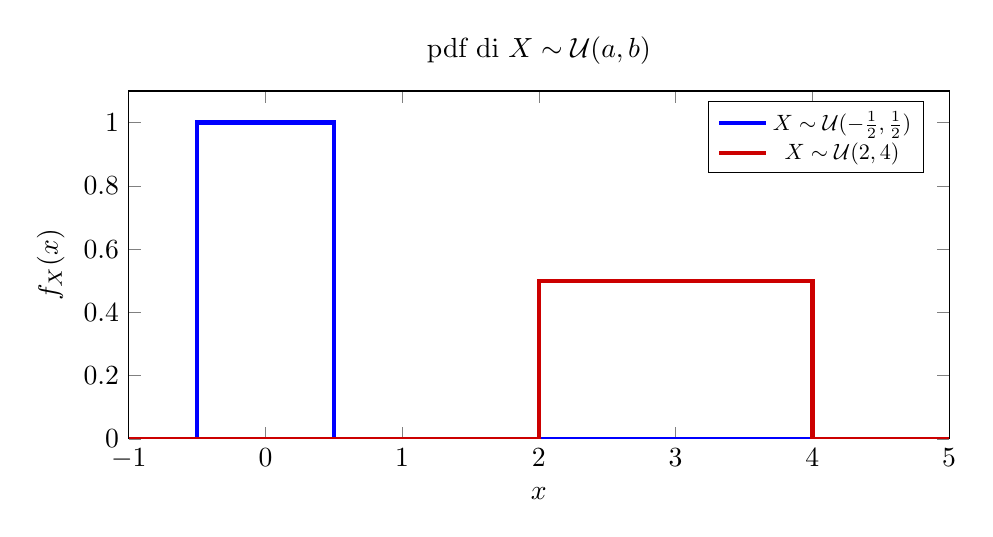
\begin{tikzpicture}
    \begin{axis}[
        width=12cm, height=6cm,
        title={pdf di $X \sim \mathcal{U}(a,b)$},
        xlabel={$x$},
        ylabel={$f_X(x)$},
        ymin=0, ymax=1.1,
        xmin=-1, xmax=5,
        legend pos=north east,
        legend style={nodes={scale=0.8, transform shape}},
        ytick={0, 0.2, 0.4, 0.6, 0.8, 1},
        xtick={-1, 0, 1, 2, 3, 4, 5}
    ]
        % U(-0.5, 0.5)
        \addplot[blue, ultra thick] coordinates {
            (-1,0) (-0.5,0) (-0.5,1) (0.5,1) (0.5,0) (5,0)
        };
        \addlegendentry{$X \sim \mathcal{U}(-\frac{1}{2}, \frac{1}{2})$}
        
        % U(2, 4)
        \addplot[red!80!black, ultra thick] coordinates {
            (-1,0) (2,0) (2,0.5) (4,0.5) (4,0) (5,0)
        };
        \addlegendentry{$X \sim \mathcal{U}(2, 4)$}
    \end{axis}
\end{tikzpicture}

\vspace{0.5cm}

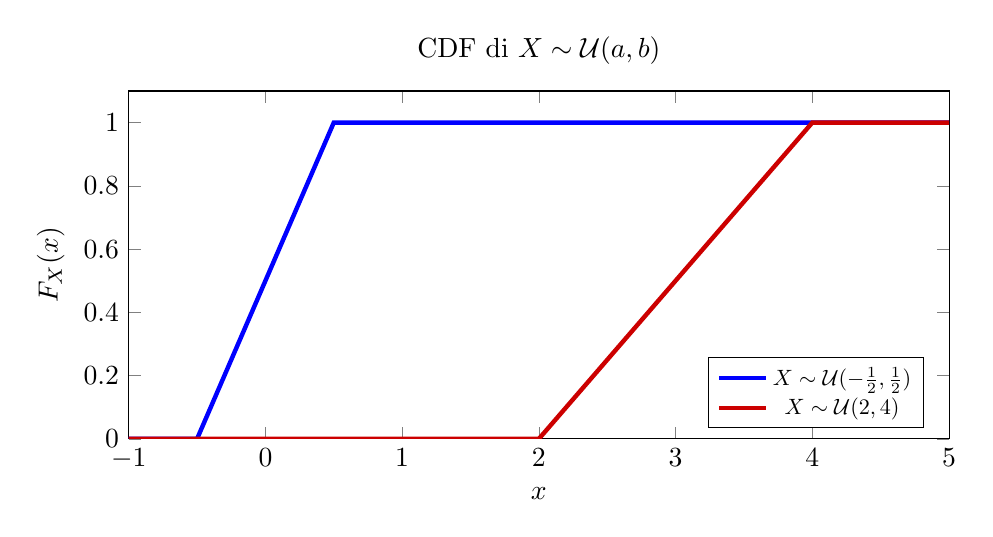
\begin{tikzpicture}
    \begin{axis}[
        width=12cm, height=6cm,
        title={CDF di $X \sim \mathcal{U}(a,b)$},
        xlabel={$x$},
        ylabel={$F_X(x)$},
        ymin=0, ymax=1.1,
        xmin=-1, xmax=5,
        legend pos=south east,
        legend style={nodes={scale=0.8, transform shape}},
        ytick={0, 0.2, 0.4, 0.6, 0.8, 1},
        xtick={-1, 0, 1, 2, 3, 4, 5}
    ]
        % U(-0.5, 0.5)
        \addplot[blue, ultra thick] coordinates {
            (-1,0) (-0.5,0) (0.5,1) (5,1)
        };
        \addlegendentry{$X \sim \mathcal{U}(-\frac{1}{2}, \frac{1}{2})$}
        
        % U(2, 4)
        \addplot[red!80!black, ultra thick] coordinates {
            (-1,0) (2,0) (4,1) (5,1)
        };
        \addlegendentry{$X \sim \mathcal{U}(2, 4)$}
    \end{axis}
\end{tikzpicture}
\end{center}

\subsection{La Distribuzione Esponenziale}

Una variabile aleatoria continua $X$ si dice \textbf{distribuita esponenzialmente} con parametro $\lambda > 0$, e si indica con la notazione $X \sim \mathcal{E}(\lambda)$, se modella fenomeni come il tempo di attesa per il verificarsi di un evento (ad esempio, il tempo di vita di un componente elettronico o l'arrivo di un cliente).

\subsubsection{1. Funzione di Densità di Probabilità (PDF)}
La PDF della distribuzione esponenziale è descritta da un decadimento esponenziale ed è definita come:

\begin{equation}
f_X(x) = \lambda e^{-\lambda x} u(x)
\end{equation}

Dove $u(x)$ è il \textbf{gradino unitario continuo} (funzione di Heaviside), che vale $1$ per $x \ge 0$ e $0$ per $x < 0$. Questo implica che il supporto della funzione è $[0, +\infty[$, ovvero la variabile $X$ può assumere solo valori non negativi ($X \ge 0$).

\subsubsection{2. Funzione di Ripartizione (CDF)}
La CDF si calcola integrando la densità di probabilità da $0$ fino a $x$. Poiché per $x < 0$ la probabilità è nulla, consideriamo solo il caso $x \ge 0$:

\begin{equation}
F_X(x) = \int_{0}^{x} \lambda e^{-\lambda t} dt = \left[ -e^{-\lambda t} \right]_{0}^{x} = (1 - e^{-\lambda x}) u(x)
\end{equation}

\subsubsection{3. Valore Atteso (Media Statistica)}
Applicando la definizione di valore atteso e integrando per parti, la media statistica risulta inversamente proporzionale al parametro $\lambda$:

\begin{equation}
\mathbb{E}[X] = \int_{0}^{+\infty} x \left(\lambda e^{-\lambda x}\right) dx = \frac{1}{\lambda}
\end{equation}

\subsubsection{Rappresentazione Grafica (Esponenziale)}

\begin{center}
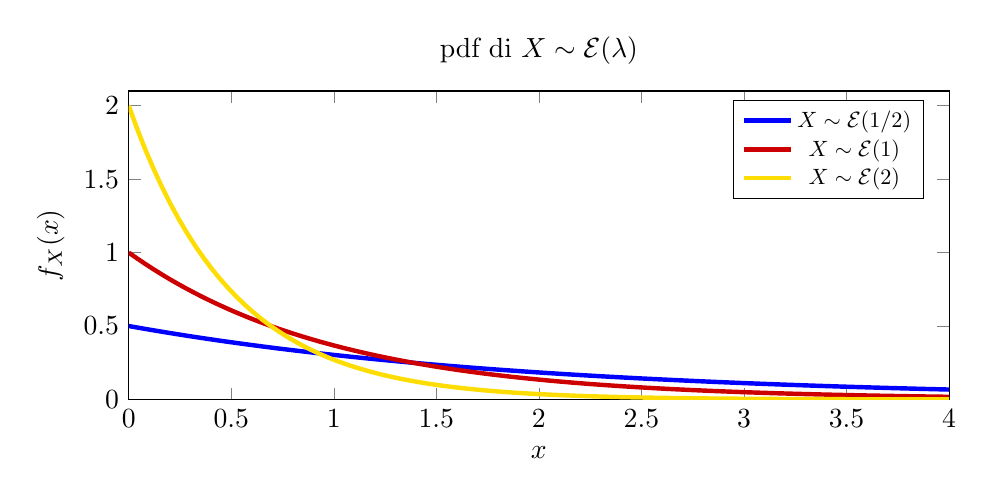
\begin{tikzpicture}
    \begin{axis}[
        width=12cm, height=5.5cm,
        title={pdf di $X \sim \mathcal{E}(\lambda)$},
        xlabel={$x$}, ylabel={$f_X(x)$},
        ymin=0, ymax=2.1, xmin=0, xmax=4,
        domain=0:4, samples=100,
        legend pos=north east,
        legend style={nodes={scale=0.8, transform shape}}
    ]
        % lambda = 0.5
        \addplot[blue, ultra thick] {0.5 * exp(-0.5 * x)};
        \addlegendentry{$X \sim \mathcal{E}(1/2)$}
        
        % lambda = 1
        \addplot[red!80!black, ultra thick] {1 * exp(-1 * x)};
        \addlegendentry{$X \sim \mathcal{E}(1)$}
        
        % lambda = 2
        \addplot[yellow!80!orange, ultra thick] {2 * exp(-2 * x)};
        \addlegendentry{$X \sim \mathcal{E}(2)$}
    \end{axis}
\end{tikzpicture}

\vspace{0.3cm}

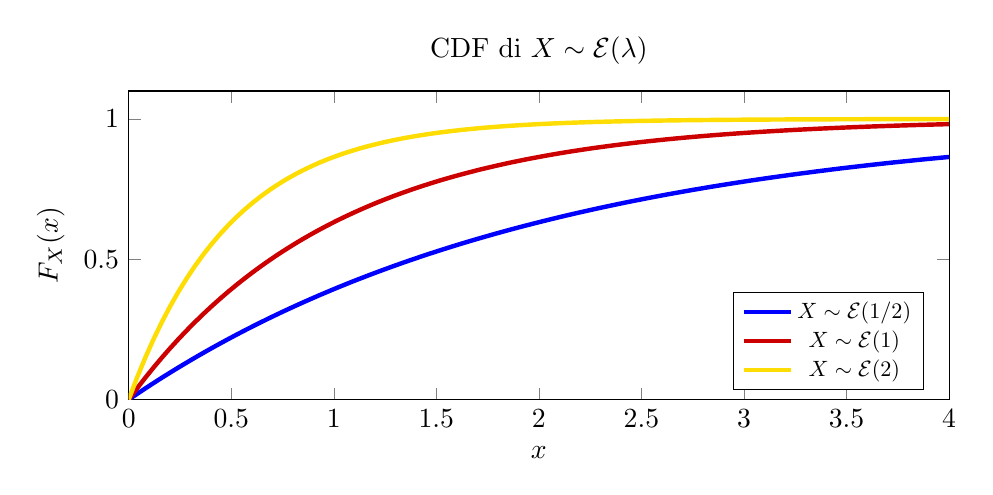
\begin{tikzpicture}
    \begin{axis}[
        width=12cm, height=5.5cm,
        title={CDF di $X \sim \mathcal{E}(\lambda)$},
        xlabel={$x$}, ylabel={$F_X(x)$},
        ymin=0, ymax=1.1, xmin=0, xmax=4,
        domain=0:4, samples=100,
        legend pos=south east,
        legend style={nodes={scale=0.8, transform shape}}
    ]
        % lambda = 0.5
        \addplot[blue, ultra thick] {1 - exp(-0.5 * x)};
        \addlegendentry{$X \sim \mathcal{E}(1/2)$}
        
        % lambda = 1
        \addplot[red!80!black, ultra thick] {1 - exp(-1 * x)};
        \addlegendentry{$X \sim \mathcal{E}(1)$}
        
        % lambda = 2
        \addplot[yellow!80!orange, ultra thick] {1 - exp(-2 * x)};
        \addlegendentry{$X \sim \mathcal{E}(2)$}
    \end{axis}
\end{tikzpicture}
\end{center}


\subsection{La Distribuzione Laplaciana}

Una variabile aleatoria continua $X$ si dice \textbf{laplaciana} (o a doppia esponenziale) con parametro $\lambda > 0$, e si indica con $X \sim \mathcal{L}(\lambda)$, quando la sua distribuzione presenta un picco al centro e decresce esponenzialmente e in modo simmetrico verso i due infiniti.

\subsubsection{1. Funzione di Densità di Probabilità (PDF)}
La PDF è definita su tutto l'asse reale (supporto $\mathbb{R}$) e utilizza il valore assoluto per garantire la simmetria:

\begin{equation}
f_X(x) = \frac{\lambda}{2} e^{-\lambda |x|}
\end{equation}

\subsubsection{2. Funzione di Ripartizione (CDF)}
Essendo presente un valore assoluto, il calcolo della CDF richiede di spezzare l'integrale in due casi distinti, a seconda che si stia integrando nella metà negativa o in quella positiva dell'asse delle ascisse:

\begin{equation}
F_X(x) = \int_{-\infty}^{x} \frac{\lambda}{2} e^{-\lambda |t|} dt = 
\begin{cases} 
\frac{\lambda}{2} \int_{-\infty}^{x} e^{\lambda t} dt = \frac{1}{2} e^{\lambda x} & \text{se } x \le 0 \\ 
\\
\frac{\lambda}{2} \left[ \int_{-\infty}^{0} e^{\lambda t} dt + \int_{0}^{x} e^{-\lambda t} dt \right] = 1 - \frac{1}{2} e^{-\lambda x} & \text{se } x > 0
\end{cases}
\end{equation}

\subsubsection{3. Valore Atteso (Media Statistica)}
La media di una variabile laplaciana è sempre nulla. Questo è un risultato immediato che vale per tutte le PDF pari (simmetriche rispetto all'asse $y$). 
Infatti, moltiplicando la funzione dispari $x$ per la funzione pari $e^{-\lambda |x|}$, si ottiene una funzione integranda dispari. L'integrale di una funzione dispari esteso da $-\infty$ a $+\infty$ vale sempre $0$:

\begin{equation}
\mathbb{E}[X] = \frac{\lambda}{2} \int_{-\infty}^{+\infty} x e^{-\lambda |x|} dx = 0
\end{equation}

\subsubsection{Rappresentazione Grafica (Laplaciana)}

\begin{center}
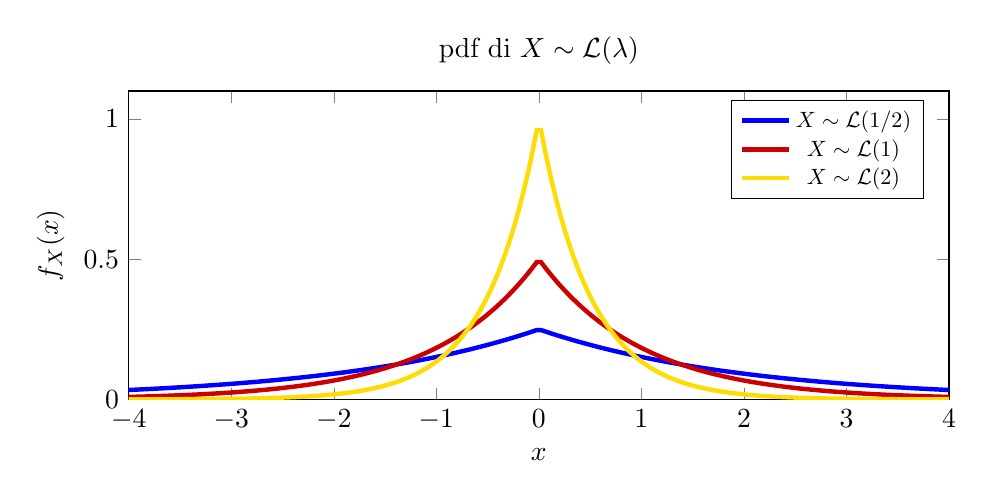
\begin{tikzpicture}
    \begin{axis}[
        width=12cm, height=5.5cm,
        title={pdf di $X \sim \mathcal{L}(\lambda)$},
        xlabel={$x$}, ylabel={$f_X(x)$},
        ymin=0, ymax=1.1, xmin=-4, xmax=4,
        domain=-4:4, samples=200,
        legend pos=north east,
        legend style={nodes={scale=0.8, transform shape}}
    ]
        % lambda = 0.5
        \addplot[blue, ultra thick] {0.25 * exp(-0.5 * abs(x))};
        \addlegendentry{$X \sim \mathcal{L}(1/2)$}
        
        % lambda = 1
        \addplot[red!80!black, ultra thick] {0.5 * exp(-1 * abs(x))};
        \addlegendentry{$X \sim \mathcal{L}(1)$}
        
        % lambda = 2
        \addplot[yellow!80!orange, ultra thick] {1 * exp(-2 * abs(x))};
        \addlegendentry{$X \sim \mathcal{L}(2)$}
    \end{axis}
\end{tikzpicture}

\vspace{0.3cm}

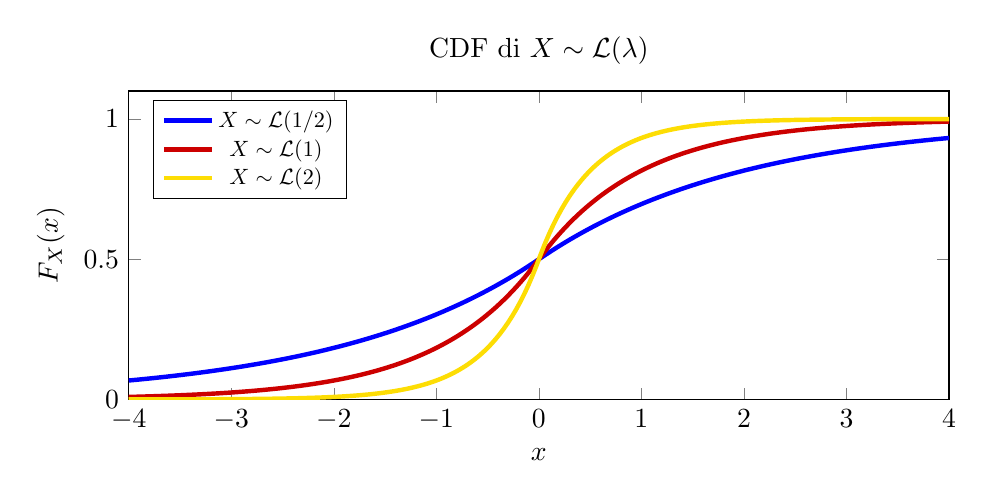
\begin{tikzpicture}
    \begin{axis}[
        width=12cm, height=5.5cm,
        title={CDF di $X \sim \mathcal{L}(\lambda)$},
        xlabel={$x$}, ylabel={$F_X(x)$},
        ymin=0, ymax=1.1, xmin=-4, xmax=4,
        domain=-4:4, samples=200,
        legend pos=north west,
        legend style={nodes={scale=0.8, transform shape}}
    ]
        % lambda = 0.5
        \addplot[blue, ultra thick] {(x<=0)*(0.5*exp(0.5*x)) + (x>0)*(1-0.5*exp(-0.5*x))};
        \addlegendentry{$X \sim \mathcal{L}(1/2)$}
        
        % lambda = 1
        \addplot[red!80!black, ultra thick] {(x<=0)*(0.5*exp(1*x)) + (x>0)*(1-0.5*exp(-1*x))};
        \addlegendentry{$X \sim \mathcal{L}(1)$}
        
        % lambda = 2
        \addplot[yellow!80!orange, ultra thick] {(x<=0)*(0.5*exp(2*x)) + (x>0)*(1-0.5*exp(-2*x))};
        \addlegendentry{$X \sim \mathcal{L}(2)$}
    \end{axis}
\end{tikzpicture}
\end{center}

\subsection{La Distribuzione di Cauchy}

Una variabile aleatoria continua $X$ si dice distribuita secondo una \textbf{distribuzione di Cauchy} (nota anche come distribuzione di Lorentz in ambito fisico) con parametri $a \in \mathbb{R}$ e $b > 0$, e si indica con $X \sim \mathcal{C}(a, b)$, se la sua densità assume la caratteristica forma a campana ma con "code" molto più spesse (pesanti) rispetto a una normale.

\begin{itemize}
    \item Il parametro $a$ rappresenta il parametro di \textbf{posizione} (indica dove si trova il picco e il centro di simmetria).
    \item Il parametro $b$ rappresenta il parametro di \textbf{scala} (regola la larghezza della campana alla sua mezza altezza).
\end{itemize}

\subsubsection{1. Funzione di Densità di Probabilità (PDF)}
La PDF è definita su tutto l'asse reale (supporto $\mathbb{R}$) ed è data dalla seguente equazione:

\begin{equation}
f_X(x) = \frac{1}{b\pi} \frac{1}{1 + \left(\frac{x-a}{b}\right)^2}
\end{equation}

Questa funzione implica che $X$ può assumere qualsiasi valore reale.

\subsubsection{2. Funzione di Ripartizione (CDF)}
Integrando la PDF da $-\infty$ a $x$, si ottiene la funzione di ripartizione. L'integrale di questa funzione fratta produce un'arcotangente:

\begin{equation}
F_X(x) = \frac{1}{b\pi} \int_{-\infty}^{x} \frac{dt}{1 + \left(\frac{t-a}{b}\right)^2} = \frac{1}{2} + \frac{1}{\pi} \arctan\left(\frac{x - a}{b}\right)
\end{equation}
Notiamo che, essendo il codominio dell'arcotangente compreso tra $(-\frac{\pi}{2}, +\frac{\pi}{2})$, il valore della CDF oscilla correttamente e in modo continuo tra $0$ e $1$.

\subsubsection{3. Valore Atteso: La particolarità di Cauchy}
La distribuzione di Cauchy è celebre in statistica per una sua anomalia matematica: \textbf{la sua media statistica non è definita}. 

Se proviamo a calcolare il valore atteso applicando la definizione formale $\mathbb{E}[X] = \int_{-\infty}^{+\infty} x f_X(x) dx$, ci accorgiamo che la funzione integranda $x f_X(x)$ non è sommabile. A causa delle "code pesanti" della curva, l'integrale diverge.

Tuttavia, poiché la distribuzione è perfettamente simmetrica rispetto al punto $a$, è possibile definire un "centro di simmetria" ricorrendo al concetto di \textbf{integrale a valore principale di Cauchy}. Calcolando il limite per un intervallo di integrazione simmetrico $[-H, H]$ che tende all'infinito, i contributi opposti si elidono, restituendo il parametro $a$:

\begin{equation}
\frac{1}{b\pi} \lim_{H \to \infty} \int_{-H}^{H} \frac{x}{1 + \left(\frac{x-a}{b}\right)^2} dx = a
\end{equation}

\textit{Attenzione:} Questo valore $a$ identifica il picco (la moda) e il punto di mezzo (la mediana), ma dal punto di vista rigoroso della teoria della probabilità, la media $\mathbb{E}[X]$ continua a non esistere.

\subsubsection{Rappresentazione Grafica (Cauchy)}

\begin{center}
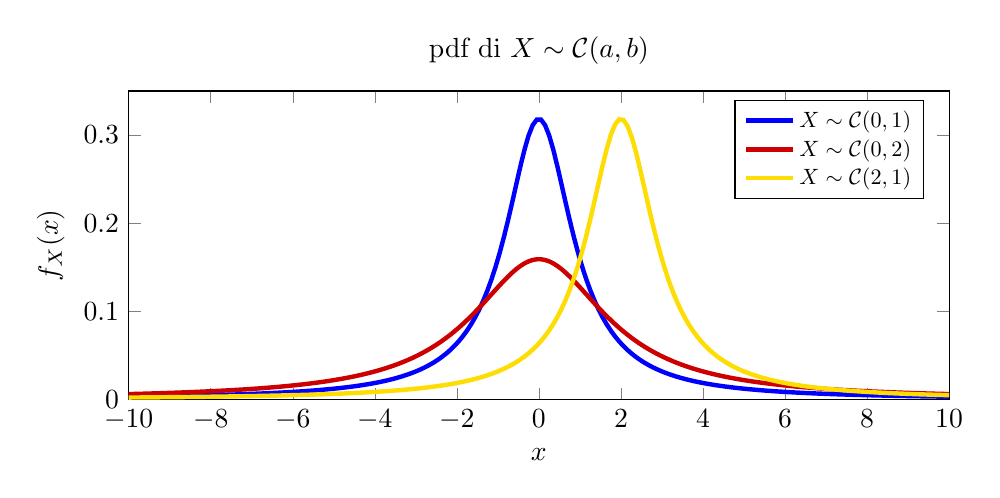
\begin{tikzpicture}
    \begin{axis}[
        width=12cm, height=5.5cm,
        title={pdf di $X \sim \mathcal{C}(a,b)$},
        xlabel={$x$}, ylabel={$f_X(x)$},
        ymin=0, ymax=0.35, xmin=-10, xmax=10,
        domain=-10:10, samples=200,
        legend pos=north east,
        legend style={nodes={scale=0.8, transform shape}}
    ]
        % C(0,1) 
        \addplot[blue, ultra thick] {1/(pi * (1 + x^2))};
        \addlegendentry{$X \sim \mathcal{C}(0,1)$}
        
        % C(0,2) 
        \addplot[red!80!black, ultra thick] {1/(2*pi * (1 + (x/2)^2))};
        \addlegendentry{$X \sim \mathcal{C}(0,2)$}
        
        % C(2,1)
        \addplot[yellow!80!orange, ultra thick] {1/(pi * (1 + (x-2)^2))};
        \addlegendentry{$X \sim \mathcal{C}(2,1)$}
    \end{axis}
\end{tikzpicture}

\vspace{0.3cm}

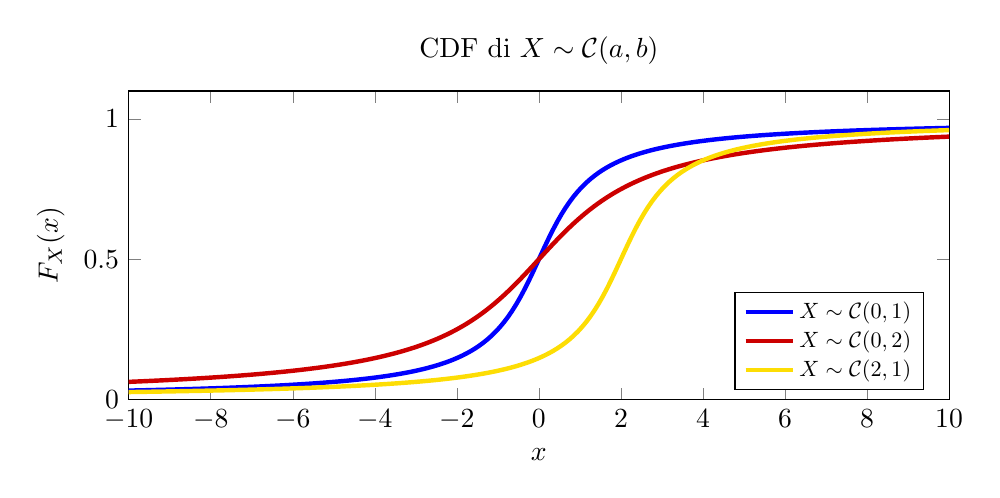
\begin{tikzpicture}
    \begin{axis}[
        width=12cm, height=5.5cm,
        title={CDF di $X \sim \mathcal{C}(a,b)$},
        xlabel={$x$}, ylabel={$F_X(x)$},
        ymin=0, ymax=1.1, xmin=-10, xmax=10,
        domain=-10:10, samples=200,
        legend pos=south east,
        legend style={nodes={scale=0.8, transform shape}}
    ]
        % C(0,1) -> (atan(x) in pgfplots gives degrees, divide by 180 to get pi fractions)
        \addplot[blue, ultra thick] {0.5 + atan(x)/180};
        \addlegendentry{$X \sim \mathcal{C}(0,1)$}
        
        % C(0,2)
        \addplot[red!80!black, ultra thick] {0.5 + atan(x/2)/180};
        \addlegendentry{$X \sim \mathcal{C}(0,2)$}
        
        % C(2,1)
        \addplot[yellow!80!orange, ultra thick] {0.5 + atan(x-2)/180};
        \addlegendentry{$X \sim \mathcal{C}(2,1)$}
    \end{axis}
\end{tikzpicture}
\end{center}